%=========================================================
\chapter{Marco Teórico}
\label{cap:reqUsr}

	Este capítulo está enfocado en detallar la información esencial para el entendimiento del Trabajo Terminal, además de explicar y establecer las tecnologías que se usarán para el desarrollo de este.
	Para comenzar
	
%---------------------------------------------------------
% !TeX root = ../ejemplo.tex

\section{Evaluaciones a Título de Suficiencia (ETS)}
En el Instituto Politécnico Nacional (IPN), incluyendo unidades académicas como la Escuela Superior de Cómputo (ESCOM), la acreditación de cada unidad de aprendizaje se realiza semestralmente a través de 3 evaluaciones ordinarias. Si un alumno no acredita alguna unidad de aprendizaje, tendrá la oportunidad de presentar una evaluación extraordinaria. Estos procedimientos están detallados en el programa de estudios y se encuentran especificados en el calendario académico.

El alumno que no logre acreditar una o más de las unidades de aprendizaje en la que se haya inscrito podrá optar por acreditarlas mediante Evaluación a Título de Suficiencia, de acuerdo con lo establecido en el Artículo 39 del Reglamento Interno del IPN, que señala: 

\begin{quote}
	``La evaluación del aprendizaje se llevará a cabo a través de exámenes ordinarios, extraordinarios y a título de suficiencia, cuyos requisitos y procedimientos de elaboración, presentación y exención, así como de otros mecanismos de evaluación continua, se realizarán en los términos que fijen los planes y programas de estudio, el presente Reglamento y los reglamentos respectivos.''
\end{quote}

Existen dos rondas de ETS:
\begin{itemize}
	\item ETS Ordinario: Esta es la primera oportunidad que tiene el alumno para acreditar la materia en la que no obtuvo una calificación aprobatoria. Los ETS ordinarios generalmente se aplican al finalizar el semestre, permitiendo al estudiante demostrar sus conocimientos sin necesidad de repetir el curso completo. 
	\item ETS Especiales: Si el alumno no acredita la materia en el ETS ordinario, puede optar por presentar un ETS Especial. Esta es la segunda oportunidad que tiene el alumno para pasar la materia. Esta evaluación adicional suele programarse el primer viernes del nuevo semestre, brindando al estudiante una opción rápida para regularizar sus situación académica y continuar avanzando en su plan de estudios. 
\end{itemize}

\subsection{Procedimiento para realizar un ETS}
\begin{itemize}
	\item Pagar en caja, verificar que estén correctos los siguientes datos: Nombre, Boleta, Carrera y Número de unidades de aprendizaje.
	\item Acudir a ventanilla de gestión escolar para generar créditos en el “SAES”.
	\item Una vez generados los créditos, inscribe las unidades de aprendizaje en la página del “SAES”.
	\item Entregar en ventanilla de gestión escolar, el comprobante de inscripción de ES generador por SAES, y el recibo de pago para dar fin a la inscripción al ETS. 
	\item  Acudir el día y la hora establecida en el calendario.
\end{itemize}
%---------------------------------------------------------
% !TeX root = ../ejemplo.tex

\section{Códigos QR}

Actualmente las credenciales del IPN incluyen un código QR que, al ser escaneado, proporcionan acceso a la información del alumno.
Este Código QR contiene datos esenciales como el nombre completo del estudiante, numero de boleta, la carrera en la que está inscrito y su fotografía. Además, en algunas unidades académicas del IPN, los códigos QR de las credenciales se utilizan como un medio de verificación de identidad para el acceso a las instalaciones mediante el uso de torniquetes electrónicos.

Para la elaboración de nuestro TT, el código QR desempeña un papel fundamental en la corroboración de la identidad de los estudiantes. Las credenciales escolares al contener un código QR se puede aprovechar la capacidad para almacenar y transmitir información de manera segura y rápida. Este enfoque nos permite verificar la información del estudiante mediante un simple escaneo, reduciendo el tiempo necesario para corroborar la identidad. Al escanear el código QR en la credencial. El sistema accede a los datos del alumno, lo cual permite verificar si coincide con la persona que se presenta al ETS.

Un código QR es un tipo de código de barras bidimensionales que solo se puede leer con teléfonos inteligentes u otros dispositivos dedicados a la lectura de estos códigos. Cuando se lee un código QR, los dispositivos se conectan directamente a mensajes de texto, correos electrónicos, sitios web, números de teléfono, etc \cite{CitaA01}.

\subsection{Anatomía de un código QR}
\title{Patrones de detección de posición}\\

\begin{figure}[htbp]
	\begin{center}
		\fbox{
\includegraphics[width=.24\textwidth]{images/img01}}
		\caption{Patrones de detección de posición \cite{CitaA01}.}
		\label{fig:Patrones de deteccion de posicion2}
	\end{center}
\end{figure}

Los patrones de detección de posición se encuentran en las tres esquinas del código. Gracias a ellos, el escáner puede reconocer y leer el código QR rápidamente. Estos marcadores indican la dirección en la que se imprimió el código QR y ayudan a su identificación y orientación. \\

\title{Patrones de alineación}

\begin{figure}[htbp]
	\begin{center}
		\fbox{
\includegraphics[width=.24\textwidth]{images/img02}}
		\caption{Patrones de alineación \cite{CitaA01}.}
		\label{fig:Patrones de alineacion1}
	\end{center}
\end{figure}

Usados para corregir la distorsión del código QR en superficies curvas. El tamaño y la cantidad de los patrones de alineación pueden variar según el volumen de la información almacenada en el código \cite{CitaA01}. \\

\title{Patrones de temporización}

\begin{figure}[htbp]
	\begin{center}
		\fbox{
\includegraphics[width=.24\textwidth]{images/img03}}
		\caption{Patrones de temporización \cite{CitaA01}.}
		\label{fig:temporizacion}
	\end{center}
\end{figure}

La alternancia de los módulos negros y blancos del código QR detrmina el sistema de información, también llamado cuadrícula de datos. Con estas líneas, el escáner reconoce la matriz de datos. 

\newpage

\title{Información sobre la versión}

\begin{figure}[htbp]
	\begin{center}
		\fbox{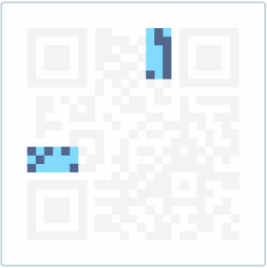
\includegraphics[width=.24\textwidth]{images/img04}}
		\caption{Información sobre la versión \cite{CitaA01}.}
		\label{fig:version}
	\end{center}
\end{figure}

Estos marcadores indican cuál de las 40 versiones del código QR está siendo usada. Normalmente las versiones utilizadas son de 1 a 7. \cite{CitaA01}\\

\title{Información del formato}

\begin{figure}[htbp]
	\begin{center}
		\fbox{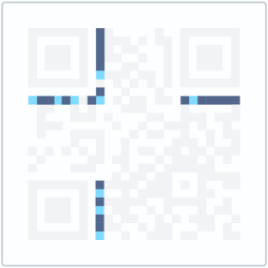
\includegraphics[width=.24\textwidth]{images/img05}}
		\caption{Información del formato \cite{CitaA01}.}
		\label{fig:formato2}
	\end{center}
\end{figure}

Contiene información sobre la tolerancia a los errores y el patrón del enmascaramiento de datos. La información sobre el formato facilita el escaneo del código. \cite{CitaA01}\\

\newpage
\title{Código de corrección de datos y errores}

\begin{figure}[htbp]
	\begin{center}
		\fbox{
\includegraphics[width=.24\textwidth]{images/img06}}
		\caption{Código de corrección de datos y errores \cite{CitaA01}.}
		\label{fig:erroresDatos}
	\end{center}
\end{figure}

El sistema de corrección de errores del código QR almacena toda la información y comparte el espacio con los módulos de corrección de errores, que permiten reconstruir los datos perdidos\cite{CitaA01} . \\

\title{Márgenes}

\begin{figure}[htbp]
	\begin{center}
		\fbox{
\includegraphics[width=.24\textwidth]{images/img07}}
		\caption{Márgenes \cite{CitaA01}}
		\label{fig:margenes}
	\end{center}
\end{figure}

Los márgenes, o también llamado zona quieta, alrededor del código QR son similares al espacio blanco en un diseño, proporcionan estructura y una mejor comprensión. Pero, ¿cómo? Para que el software de escaneo identifique bien el límite del código QR de sus alrededores, los márgenes son vitales.

\subsection{Fiabilidad de los códigos QR}
Los códigos QR están diseñados para mantener la información legible, aunque estén oscuros o dañados. Esto se logra mediante la compensación de errores, es decir, insertando la información varias veces. Con un alto nivel de seguridad, los códigos QR pueden leerse incluso si un tercio de su información es ilegible. Esto hace que los códigos QR sean muy fiables a la hora de guardar información. \\


%---------------------------------------------------------
% !TeX root = ../ejemplo.tex

\section{Aplicación móvil}
Una aplicación móvil, es un tipo de aplicación diseñada para ejecutarse en un dispositivo móvil, que puede ser un teléfono inteligente. A  diferencia de las aplicaciones diseñadas para computadoras de escritorio, las aplicaciones móviles se alejan de los sistemas de software integrados. \\

Debido a los recursos de hardware limitados de los primeros dispositivos móviles, las aplicaciones móviles evitaban la multifuncionalidad. Sin embargo, incluso si los dispositivos que se utilizan hoy en día son mucho más sofisticados, las aplicaciones móviles siguen siendo funcionales. Así es como los propietarios de aplicaciones móviles permiten a los consumidores seleccionar exactamente las funciones que deben tener sus dispositivos \cite{IM1}. \\

Existen diferentes tipos de aplicaciones móviles que responden a las necesidades y preferencias de los usuarios, así como a las capacidades técnicas de los dispositivos. A continuación, se detallan cada uno:

\begin{figure}[htbp]
	\begin{center}
		\fbox{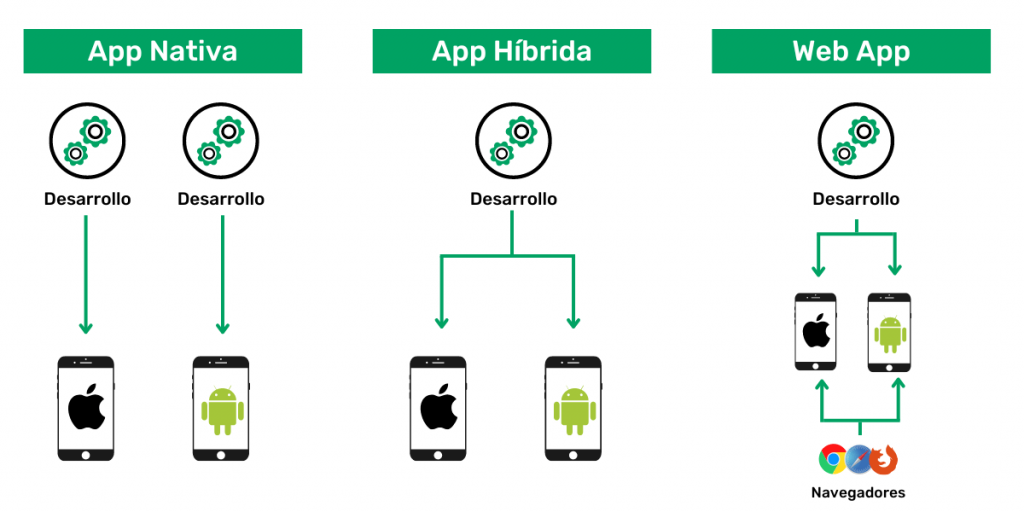
\includegraphics[width=.68\textwidth]{images/img08}}
		\caption{Tipo de aplicaciones moviles \cite{IM1}.}
		\label{fig:casosDeUso}
	\end{center}
\end{figure}

\subsection{Aplicaciones nativas}
Las aplicaciones nativas son apps desarrolladas para un sistema operativo móvil concreto (iOS o Android normalmente), en el lenguaje de programación específico de cada plataforma. Esto quiere decir que una app nativa creada para Android no puede ser utilizada en un dispositivo iOS y viceversa. \\

Es el tipo de aplicación móvil más conocida. Para que funcione, debemos descargarla desde los markets de apps, como App Store o Google Play e instalarla en nuestro teléfono \cite{CitaA02}.

\subsection*{Ventajas}
\begin{itemize}
	\item \textbf{Tienen el mejor rendimiento.} Las aplicaciones nativas son las más rápidas y tienen un rendimiento superior a otros tipos de apps, ya que han sido optimizadas específicamente para el hardware y el sistema operativo del dispositivo.
	\item \textbf{Acceso completo e integración con las funciones hardware del dispositivo.} Las apps nativas permiten aprovechar al máximo las funcionalidades móviles: cámara, micrófono, lector biométrico de huella, sensores y redes inalámbricas.
	\item \textbf{Pueden funcionar sin acceso a internet (funcionamiento offline)} si han sido diseñadas para ello.
\end{itemize}

\subsection*{Desventajas}
\begin{itemize}
	\item \textbf{Costes de desarrollo altos.} Si queremos tener nuestra app disponible para los dos sistemas, necesitaremos dos líneas de desarrollo diferentes, ya que el código utilizado para un sistema no es reutilizable para otro.
	\item \textbf{Complejidad de desarrollo.} Necesitamos equipos expertos en el lenguaje específico de cada sistema. Por ejemplo, en Kotlin para Android y en Swift para iOS.
	\item \textbf{Tiempo de desarrollo superior.} El desarrollo puede tomar entre 4 a 6 meses.
\end{itemize}

\subsection{Aplicaciones Web}

Las aplicaciones web realmente son webs especiales diseñadas para navegadores móviles. A diferencia de las apps nativas o híbridas, no necesitan ser descargadas, ya que se accede a ellas desde un navegador web.

Emplean las mismas tecnologías de desarrollo que una web, como HTML, CSS o JavaScript. Así, estaríamos hablando de una web con apariencia de app, por lo que presentaría sus mismas limitaciones. Sin embargo, con la llegada del HTML5, se han conseguido salvar algunas limitaciones, como el acceso a algunas funciones del móvil (geolocalización, cámaras) \cite{IM1}.

\subsection*{Ventajas}
\begin{itemize}
	\item \textbf{Carácter multiplataforma.} Con una sola línea de desarrollo.
	\item \textbf{Fácil desarrollo.} Se emplean tecnologías ampliamente conocidas.
	\item \textbf{Tiempo y coste de desarrollo bajo.}
\end{itemize}

\subsection*{Desventajas}
\begin{itemize}
	\item \textbf{Acceso limitado a las funciones del dispositivo.}
	\item \textbf{No se pueden subir a las tiendas de aplicaciones.}
	\item \textbf{Diferentes experiencias de usuario.} Estas dependen del navegador utilizado.
	\item \textbf{Necesidad de conexión a Internet.} Incluso si se cuenta con un modo pensado para ello, es necesario para acceder a las posibles actualizaciones o para entrar por primera vez.
\end{itemize}

\subsection{Aplicaciones Híbridas}

Las aplicaciones híbridas o multiplataforma combinan elementos de las aplicaciones nativas y las aplicaciones web. Estas aplicaciones se desarrollan utilizando tecnologías web como HTML, CSS y JavaScript, pero se empaquetan en un formato que puede ser instalado en un dispositivo móvil como cualquier otra aplicación nativa. Por tanto, podemos obtener una aplicación para varias plataformas con un único desarrollo \cite{IM1}.

\subsection*{Ventajas}
\begin{itemize}
	\item \textbf{Menor coste.} Gracias al uso de lenguajes de programación más conocidos, con una mayor disponibilidad de profesionales en el mercado.
	\item \textbf{Carácter multiplataforma.} Con una sola línea de desarrollo.
	\item \textbf{Acceso a algunas funcionalidades del móvil.}
	\item \textbf{Reducción de los tiempos de desarrollo.} Generalmente, el tiempo de desarrollo se reduce a 3 meses.
	\item \textbf{Disponibilidad en markets.} Se pueden subir a los markets de aplicaciones, como App Store y Google Play.
\end{itemize}

\subsection*{Desventajas}
\begin{itemize}
	\item \textbf{Rendimiento inferior.} Su rendimiento es inferior al de una app nativa, suelen tener un tamaño considerable y, además, ser más lentas.
	\item \textbf{Acceso limitado a las funciones del dispositivo.}
\end{itemize}

\subsection{Aplicaciones Progresivas Web Apps (PWA)}

Las aplicaciones progresivas son un reciente avance de las Web Apps. Al igual que las Web Apps, son webs diseñadas para móviles, pero esta vez, sí pueden ser descargadas en el móvil como una aplicación más, aunque no es necesario para que ofrezcan un comportamiento similar al de una app nativa a través del navegador. \\

Las PWA adoptan un comportamiento más propio de aplicaciones nativas que de web, como el funcionamiento sin Internet, un mayor rendimiento o su funcionamiento en segundo plano. Sin embargo, como desventaja, seguimos contando con la imposibilidad de subirlas a los markets de aplicaciones \cite{IM1}. \\

Para comprender mejor las diferencias entre los tipos de aplicaciones móviles, a continuación se presenta una tabla comparativa que destaca sus características clave:
\newpage

\begin{table}[h!]
	\centering
	\begin{tabular}{|p{4cm}|p{2cm}|p{2cm}|p{2cm}|}
		\hline
		\textbf{Tipos de app} & \textbf{Nativa} & \textbf{Híbrida} & \textbf{Web} \\ \hline
		\textbf{Interfaz} & Basada en web & Específica de la plataforma (iOS, Android) & Basada en web \\ \hline
		\textbf{Tiempo de desarrollo} & Alto & Medio & Bajo \\ \hline
		\textbf{Coste de desarrollo} & Alto & Medio & Bajo \\ \hline
		\textbf{Multiplataforma} & No & Sí & Sí \\ \hline
		\textbf{Rendimiento} & Alto & Medio & Bajo \\ \hline
		\textbf{Acceso a los sensores del dispositivo} & Completo & Alto o Completo & Limitado \\ \hline
		\textbf{Tiendas de aplicaciones} & Sí & Sí & No \\ \hline
	\end{tabular}
	\caption{Comparación tipos de aplicaciones móviles. Elaboración propia}
	\label{tab:tipos_apps}
\end{table}

Para el desarrollo de nuestro trabajo terminal, hemos decidido optar por una aplicación híbrida con el uso de Kotlin. Esta decisión se basa en varios factores relacionados con los recursos disponibles, las características de nuestro público objetivo y los plazos establecidos. \\

La aplicación móvil está dirigida para estudiantes, alumnos y personal de seguridad de la Escuela Superior de Cómputo, donde la mayoría utiliza dispositivos con sistema operativo Android. La elección de una aplicación híbrida nos permite optimizar  la experiencia en Android, que es la plataforma que predomina entre nuestros usuarios. \\

Aunque las aplicaciones híbridas suelen desarrollarse con tecnologías web (como React Native o Flutter), para nuestro proyecto hemos decidido incorporar Kotlin para desarrollar modelos donde se requiera un rendimiento nativo o un acceso más profundo a las funciones del sistema operativo Android.Además, las aplicaciones híbridas permiten un desarrollo más rápido en comparación con las aplicaciones completamente nativas, ya que gran parte del código puede compartirse entre plataformas, así mismo, es una buena opción económica que se adapta a nuestro presupuesto \cite{IM1}. 


%---------------------------------------------------------
% !TeX root = ../ejemplo.tex

\section{Sistema operativo}

%---------------------------------------------------------
% !TeX root = ../ejemplo.tex

\section{Lenguaje de programación}

%---------------------------------------------------------
% !TeX root = ../ejemplo.tex

\section{Framework}
\subsection{Jetpack compose}
Para la implementación de la aplicación móvil que forma parte de nuestro sistema de identificación y control de acceso, hemos decidido utilizar Jetpack Compose. La elección de la tecnología adecuada es importante para ofrecer una mejor experiencia de usuario y cumplir nuestros objetivos de diseño y funcional. 

\subsection*{¿Por que Jetpack compose?}
Jetpack compose es un framework (estructura o marco de trabajo que, bajo parámetros estandarizados, ejecutan tareas específicas en el desarrollo de un software) con la particularidad de ejecutar prácticas modernas en los desarrolladores de software a partir de la reutilización de componentes, así como también contando con la oportunidad de crear animaciones y temas oscuros. En este sentido, Jetpack Compose es el conjunto de herramientas ofrecidas por Android para el desarrollo de aplicaciones con un objetivo específico: simplificar y optimizar los códigos en la IU nativas \cite{CitaA01}. 


\subsection*{Ventajas}

\begin{itemize}
	\item \textbf{Menos código:} Simplifica el proceso de desarrollo haciendo menos código, todo se basa en funciones de modo que el código será simple y fácil de mantener.
	\item \textbf{Intuitiva:} Tan solo describe tu IU con un enfoque declarativo haciendo “qué hay que hacer” en vez de “cómo se debe hacer”.
	\item \textbf{Potente:} Tiene integrado Material Design con el cual puede crear apps atractivas al usuario con animaciones y mucho más.
	\item \textbf{Acelera el desarrollo:} Es compatible con proyectos existentes, puedes empezar a integrarlo por partes cuando quieras y donde quieras.
	\item \textbf{Kotlin:} Está escrito 100\% en Kotlin, lo cual nos permitirá usar sus herramientas potentes y API’s intuitivas.
\end{itemize}
%---------------------------------------------------------
% !TeX root = ../ejemplo.tex


\subsection{XML}
Para este proyecto utilizaremos XML debido a la múltiples ventajas que ofrece en el desarrollo de interfaces de usuario en aplicaciones web y Android\cite{CitaA03} .  

\subsection*{¿Por que XML?}

XML son siglas de \textit{Extensible Markup Language}, es un lenguaje de marcado que proporciona reglas para definir cualquier dato.

Por ejemplo, imaginemos un documento de texto con comentarios. Los comentarios pueden ofrecer sugerencias como las siguientes:
\begin{itemize}
	\item Ponga el título en negrita.
	\item Esta oración es un encabezado.
	\item Esta palabra es del autor.
\end{itemize}

Estos comentarios mejoran la usabilidad del documento sin repercutir en su contenido. Del mismo modo, XML utiliza símbolos de marcado para proporcionar más información sobre los datos.

\subsection*{Etiquetas XML}

Los s\'{\i}mbolos de marcado, denominados \textbf{etiquetas} en XML, se utilizan para definir los datos. Por ejemplo, para representar los datos de una librer\'{\i}a, se pueden crear etiquetas como:

\texttt{\textless libro\textgreater}, \texttt{\textless t\'{\i}tulo\textgreater} y \texttt{\textless autor\textgreater}

El documento XML de un solo libro tendr\'{\i}a el siguiente contenido:

\begin{lstlisting}
	<libro>
	<titulo>Introduccion a Amazon Web Services</titulo>
	<autor>Mark Wilkins</autor>
	</libro>
\end{lstlisting}


Las etiquetas ofrecen una sofisticada codificaci\'{o}n de datos para integrar los flujos de informaci\'{o}n en diferentes sistemas \cite{CitaA04}.

\subsection*{Ventajas de XML}

\begin{itemize}
	\item \textbf{Flexibilidad:} El formato XML es un lenguaje de marcas que se puede personalizar para diferentes prop\'{o}sitos.
	\item \textbf{Interoperabilidad:} El formato XML es compatible con una amplia gama de sistemas y aplicaciones, lo que significa que los datos se pueden intercambiar f\'{a}cilmente entre diferentes sistemas.
	\item \textbf{Legibilidad:} El formato XML es f\'{a}cil de leer y entender, lo que facilita la creaci\'{o}n y el mantenimiento de archivos XML.
	\item \textbf{Reutilizaci\'{o}n:} Los elementos y atributos de un archivo XML se pueden reutilizar en diferentes partes del archivo, lo que ahorra tiempo y reduce errores.
\end{itemize}
%---------------------------------------------------------
% !TeX root = ../ejemplo.tex

\section{Patrones de arquitectura de software}
Al momento de desarrollar software, es común toparnos con problemáticas que requieren de la toma de decisiones especialmente cuando hablamos sobre cuestiones relacionadas con el diseño de un sistema de software.
Un patrón de arquitectura de software es un conjunto de decisiones tomadas para atacar problemáticas relacionadas con el diseño de un software. Estos incluyen reglas y principios para organizar las interacciones entre subsistemas predefinidos y los roles que estos desempeñan \cite{L07}.

A menudo pueden ser descritos como los \textit{"Planos"} de un sistema, sin embargo, esto no quiere decir que sea la arquitectura final, sino que funcionan como una guía que describe los elementos necesarios para diseñar la arquitectura de la solución a desarrollar, la selección de una arquitectura sobre otra dependerá completamente de los objetivos a alcanzar, los recursos disponibles y la experiencia del equipo de desarrollo \cite{L08}.

Es necesario aclarar que, los patrones de arquitectura no deben confundirse con los patrones de diseño, ya que ambos responden a problemas diferentes durante el desarrollo de un sistema de software, de forma muy breve un patrón de arquitectura describe como crear la lógica de negocio, acceso a los datos, etc. Mientras que los patrones de diseño se usan al implementar estos elementos \cite{L07}.

A continuación, se describen algunos patrones de arquitectura que pueden ser de utilidad al implementar la propuesta de solución para este trabajo terminal.	

\subsection{Arquitectura de capas}

También conocida como \textit{arquitectura de N-capas}, estructura una aplicación en múltiples capas distintas, donde cada una esta encargada de ciertas tareas en especifico, lo que permite dividir un sistema en componentes aislados, lo que facilita el desarrollo rápido de aplicaciones ya que los cambios realizados en una capa no deberían afectar la lógica de las demás \cite{L09}.

Las arquitecturas basadas en este patrón suelen implementar cuatro capas distintas, la capa de presentación, la capa de negocio, de persistencia y de base de datos, sin embargo, y como es de esperarse, la arquitectura de un sistema basado en este patrón puede tener algunas diferencias en el número y tipo de capas que se implementan, por ejemplo, algunas pueden implementar capas de aplicación, servicio o acceso a datos \cite{L07}.

\subsection{Arquitectura orientada a servicios}

Las aplicaciones diseñadas siguiendo este patrón de arquitectura implementan una colección de servicios poco acoplados que se comunican entre sí a través de una red.
Cada uno de los servicios que conforman al sistema se encarga de llevar acabo una función del negocio en específico que después pueden ser requeridos por otro servicio o cliente \cite{L09}.


\subsection{Arquitectura de micro servicios}

Es una arquitectura que combina patrones de diseño para crear múltiples servicios que trabajan de forma independiente y que en conjunto forman la lógica de una aplicación. Es una alternativa a las aplicaciones monolíticas y de la arquitectura basada en servicios, en donde cada servicio esta orientado a implementar partes muy puntuales de la lógica de negocio \cite{L08}.

Su principal ventaja radica en que debido a que sus componentes se encuentran poco acoplados pueden ser desarrollados, desplegados y probados de forma independiente \cite{L09}.

La principal desventaja de este tipo de arquitectura es que puede llegar a ser compleja de implementar ya que requiere de definir la granularidad correcta de los servicios y establecer una comunicación efectiva entre estos \cite{L07}.

\subsection{El patrón modelo vista controlador}

Este patrón divide divide una aplicación en tres componentes interconectados. El modelo, la vista y el controlador. Esta separación permite organizar el código al desacoplar la lógica del negocio, interfaz de usuario y el manejo de las entradas de los usuarios, lo que a su vez promueve la modularidad, mantenibilidad y escalabilidad \cite{L09}. 

El modelo contiene los datos y lógica de negocio de la aplicación. Se encarga de regresar, almacenar y procesar la información.

La vista, también conocida como interfaz de usuario (UI) despliega la información al usuario y responde a las interacciones del usuario.

El controlador funciona como un intermediario entre el modelo y la vista. Se encarga de gestionar las entradas del usuario, actualizar el modelo y la vista para reflejar los cambios realizados en el modelo \cite{L08}.

%---------------------------------------------------------
% !TeX root = ../ejemplo.tex

\section{Redes neuronales artificiales}

Una red neuronal artificial es una técnica para la creación de programas de computación que son capaces de aprender de los datos. Se basa en el conocimiento actual sobre como funciona el cerebro humano. 
Consisten en un conjunto de nodos o neuronas interconectados entre sí que procesan y aprenden de los datos con los que cuentan, lo que permite llevar a cabo tareas como el reconocimiento de patrones y la toma de decisiones en el aprendizaje de máquina \cite{L10}.


\subsection{Estructura de una red neuronal artificial}
Toda red neuronal esta formada por capas de nodos, o neuronas artificiales, una capa de entrada, una o más capas ocultas y una capa de salida. Cada nodo se conecta a los demás y tiene un peso y un umbral determinado.
A continuación se describe el papel que cada una de estas capas en la arquitectura de una red neuronal común \cite{L11}.

\subsubsection{Capa de entrada}
La capa de entrada es responsable de recibir los datos iniciales en forma de vectores. Cada neurona en esta capa corresponde a una característica del conjunto de datos \cite{L12}.

\subsubsection{Capas ocultas}
Las capas ocultas son el núcleo de las RNA y donde ocurre el procesamiento de los datos. Estas capas aplican transformaciones no lineales mediante funciones de activación, como \textit{ReLU}, \textit{sigmoide}, o \textit{tangente hiperbólica}. El número y tamaño de las capas ocultas determinan la capacidad de la red para modelar patrones complejos \cite{L12}.

\subsubsection{Capa de salida}
La capa de salida genera los resultados finales del modelo. Para tareas de clasificación, por ejemplo, esta capa utiliza funciones como \textit{softmax} para proporcionar probabilidades asociadas a cada clase \cite{L12}.

\section{Proceso de aprendizaje}
Como ya se mencionó con anterioridad, una red neuronal es un sistema complejo que busca imitar la forma en la que el cerebro humano aprende \cite.
Este proceso de aprendizaje se realiza en dos fases conocidas como \textit{backpropagation} y \textit{forward propagation} \cite{L12}:


\subsection{Forward propagation}

\begin{itemize}
	\item \textbf{Capa de entrada:} La capa de entrada contiene nodos que representan cada característica del conjunto de datos inicial. Estos nodos reciben y procesan los datos de entrada.  
	\item \textbf{Pesos y conexiones:} Los pesos asignados a cada conexión entre neuronas determinan la influencia de una neurona sobre otra. Durante el entrenamiento, estos valores se actualizan constantemente para optimizar el rendimiento de la red.  
	\item \textbf{Capas ocultas:} Las neuronas en las capas ocultas combinan las entradas recibidas al multiplicarlas por sus respectivos pesos y sumarlas. Posteriormente, aplican una función de activación que introduce no linealidad, lo que permite identificar relaciones complejas en los datos.  
	\item \textbf{Capa de salida:} Este proceso se repite hasta llegar a la capa de salida, donde se genera el resultado final de la red neuronal.
\end{itemize}



\subsection{Backpropagation}

\begin{itemize}
	\item \textbf{Cálculo del error:} La salida generada por la red se compara con los valores esperados utilizando una función de pérdida. Para problemas de regresión, se emplea comúnmente el \textit{Error Cuadrático Medio} (\textit{Mean Squared Error, MSE}), que calcula la diferencia entre las predicciones y los valores reales:  
	$ {MSE} = \frac{1}{n} \sum_{i=1}^{n} (y_i - \hat{y}_i)^2 $
	
	\item \textbf{Optimización por descenso de gradiente:} Para reducir el error, la red emplea el algoritmo de descenso de gradiente. Este ajusta los pesos calculando la derivada de la función de pérdida con respecto a cada peso, guiando los ajustes necesarios para minimizar el error.  
	
	\item \textbf{Ajuste de pesos:} Este proceso de actualización de pesos se realiza en sentido inverso a través de toda la red, lo que permite optimizar las conexiones entre neuronas.  
	
	\item \textbf{Proceso iterativo de entrenamiento:} Durante el entrenamiento, los pasos de propagación hacia adelante, cálculo del error y retropropagación se repiten varias veces con diferentes muestras de datos, permitiendo que la red refine sus parámetros y aprenda patrones específicos.
\end{itemize}


\subsection{Funciones de activación}
Las funciones de activación son fundamentales para introducir no linealidad en el modelo. Ejemplos comunes incluyen la función \textit{ReLU} (Rectified Linear Unit) y la sigmoide. Estas funciones determinan si una neurona se activa, lo que depende del valor ponderado de sus entradas.


\section{Tipos de redes neuronales}

Las redes neuronales pueden clasificarse en distintos tipos, cada uno diseñado para cumplir propósitos específicos. Aunque no se trata de una lista exhaustiva, a continuación se describen algunas de las variantes más comunes y sus casos de uso principales \cite{L11}:


\subsection{Perceptrón} 
El perceptrón es la red neuronal más antigua, desarrollada por Frank Rosenblatt en 1958. Es el precursor de las redes neuronales modernas.  

\subsection{Perceptrón multicapa} 
También conocidas como \textit{feedforward neural networks}, estas redes están formadas por una capa de entrada, una o más capas ocultas y una capa de salida. Aunque frecuentemente se les llama MLPs, técnicamente están compuestas por neuronas sigmoides y no por perceptrones simples, ya que los problemas del mundo real suelen ser no lineales. Estas redes se entrenan alimentándolas con datos y son la base de aplicaciones como visión por computadora, procesamiento de lenguaje natural y otros modelos avanzados.

\subsection{Redes neuronales convolucionales} 
Las redes neuronales convolucionales (\textit{Convolutional Neural Networks}, CNNs) son una variante de las redes de avance directo que se utilizan principalmente en tareas como el reconocimiento de imágenes, el análisis de patrones y la visión por computadora. Estas redes aplican principios del álgebra lineal, en particular la multiplicación de matrices, para identificar patrones dentro de las imágenes.

\subsection{Redes neuronales recurrentes} 
Las redes neuronales recurrentes (\textit{Recurrent Neural Networks}, RNNs) se caracterizan por tener lazos de retroalimentación en su estructura. Estas redes son especialmente útiles para trabajar con datos temporales, donde las predicciones dependen de la información previa. Por ejemplo, se aplican en la predicción de mercados financieros y en la proyección de ventas.


\section{Limitaciones}
Las RNA tienen la capacidad de capturar patrones complejos en grandes volúmenes de datos. Sin embargo, también presentan desafíos como \cite{L13}:

\begin{itemize}
	\item \textbf{Necesidad de datos:} Requieren grandes cantidades de datos etiquetados para entrenarse adecuadamente.
	\item \textbf{Costo computacional:} Su entrenamiento puede ser intensivo en términos de tiempo y recursos computacionales.
	\item \textbf{Interpretabilidad:} Las predicciones de las RNA suelen ser difíciles de interpretar, lo que plantea retos en aplicaciones críticas.
\end{itemize} 


%---------------------------------------------------------
% !TeX root = ../ejemplo.tex

\section{Reconocimiento facial}

El reconocimiento facial es una técnica que permite a las computadoras predecir la identidad de una persona desde una imagen \cite{L14}.

Tiene múltiples aplicaciones en la industria como el desarrollo de sistemas de asistencia, en la salud, sistemas de seguridad, etc \cite{L15}. 

\subsection{Fundamentos del reconocimiento facial}

A menudo, los términos verificación de rostros e identificación de rostros se usan de forma indistinta, sin embargo, aunque ambos comparten el mismo dominio del problema, lo abordan de forma distinta \cite{L16}.

Para entender mejor la diferencia entre ambas tareas y su papel en el desarrollo de un sistema de reconocimiento facial, es que se presentan las técnicas más comunes que lo conforman \cite{L15}.

\subsubsection{Detección de rostros}

En este paso se incluyen algunas estrategias de preprocesamiento que permiten obtener imágenes de buena calidad para los métodos de extracción de características.
Aquí se localiza la región del rostro en una imagen o video y, dependiendo del contexto es posible aplicar técnicas de alineación o cortado de la imagen para aislar los elementos del fondo. Algoritmos como \textit{Viola-Jones} y modelos basados en \textit{Deep Learning}, como \textit{Multi-task Cascaded Convolutional Networks} (MTCNN), son ampliamente utilizados para esta tarea \cite{L16}. 

\subsubsection{Extracción de características}

Una vez que se tiene localizado el rostro se procede a extraer las características de este. En sistemas tradicionales, solían utilizarse descriptores como Histogramas de Gradientes Orientados (\textit{HOG}) o Escalas de Características Invariantes (\textit{SIFT}). Actualmente, los modelos basados en las redes neuronales profundas, especialmente, las redes neuronales convencionales (CNN), como \textit{FaceNet}, generan representaciones compactas conocidas como embeddings, que capturan la información más relevante del rostro \cite{L14}.

\subsubsection{Comparación y verificación}

Los embeddings faciales obtenidos se comparan con una base de datos utilizando medidas de similitud como la distancia coseno o euclidiana. Este paso permite determinar si dos rostros corresponden a la misma persona (verificación) o identificar a una persona entre múltiples registros (identificación) \cite{L14}.


\subsection{Identificación de rostros}

Como ya se mencionó, la identificación de rostros y la verificación de rostros son dos tareas distintas involucradas al momento de implementar un sistema de reconocimiento facial \cite{L14}.

La identificación facial se refiere a la tarea de identificar la identidad de una persona dada una imagen.La imagen se ingresa por un extractor de características para obtener una representación $f$. Luego, esta representación, entra a una red de clasificación para asignar la identidad asociada a la imagen de entrada \cite{L15}.

La identificación de rostros es una tarea de clasificación, por lo que los sistemas de reconocimiento facial basados en esta tarea son entrenados usando la función \textit{softmax} y la pérdida de entropía cruzada [4].

\subsection{Verificación de rostros}

Contrario a la identificación de rostros, la verificación de rostros busca verificar que dos imágenes pertenecen a la misma entidad \cite{L14}. Por lo tanto, en un sistema de reconocimiento facial basado en la verificación de rostros recibe como entrada una imagen $x$ y el identificador del rostro a ser identificado y la salida es una decisión binaria sobre si la imagen $x$ pertenece a la persona con el identificador dado \cite{L15}.

Este enfoque requiere de un proceso de extracción de características de los rostros de las personas que queremos que el sistema verifique y, por lo tanto, almacenar dichas representaciones en una base de datos \cite{L15}.

\subsection{Identificación mediante verificación}
En los sistemas tradicionales de identificación, se entrena un clasificador con $K$ clases para asignar a cada rostro de entrada una identidad específica de entre $K$ personas en la base de datos. Sin embargo, este enfoque presenta limitaciones de escalabilidad, ya que al agregar una nueva persona, es necesario reentrenar completamente el sistema con $K+1$ clases. Esto ocurre porque el clasificador inicial tiene $K$ neuronas, pero para incluir una nueva identidad, se requiere un clasificador con $K+1$ neuronas \cite{L15}.

\vspace{\baselineskip}

Para abordar este problema, un enfoque más eficiente y escalable es utilizar la comparación basada en similitud, propia de los algoritmos de verificación. En este caso, dado un rostro de entrada $x$, se ejecuta el algoritmo de verificación $K$ veces, una para cada rostro almacenado en la base de datos. La identidad del rostro de entrada se asigna a la correspondiente al ID para el cual el algoritmo de verificación indica una coincidencia \cite{L15}.

Por lo tanto, la ventaja de este tipo de enfoque híbrido radica en el hecho de que es posible agregar nuevas entidades al sistema sin la necesidad de re-entrenar los modelos de deep learning utilizados para la generación de los vectores de características de los rostros, más aún si se combina con algún tipo de mecanismo de almacenamiento de estos como las bases de datos vectoriales para acelerar el proceso de inferencia \cite{L17}.





